\par The challenges underlying FMRI preprocessing include reforming the data to be properly representative of the subject, by correcting for inconsistencies in the data. Sources of these include temporal delays in scanning, spatial inconsistencies in subject location during imaging, and random noise from equipment and background during scanning. In the case of our fMRI data, spatial variability has been accounted for and corrected by the curators.

\subsubsection{Exploratory Analysis}
\par We first looked at different measures of spread such as IQR, standard deviation, and RMS for each voxel across time. The following plots (Figure 3 and Figure 4) below show the standard deviation and RMS differences of the voxel-time courses. Interesting to note is that the outliers seem to have, to some degree, structure in their location; the outliers seem to clump together in certain places. 
\par We also had to deal with the overlap of movie scenes. More specifically, during the beginning of a new segment/run, researchers replayed the last six seconds of the audiotape of the previous run. To deal with this, we dropped the last four volumes for runs two through seven. 

\begin{figure}[H]
\centering
\begin{minipage}{.5\textwidth}
  \centering
  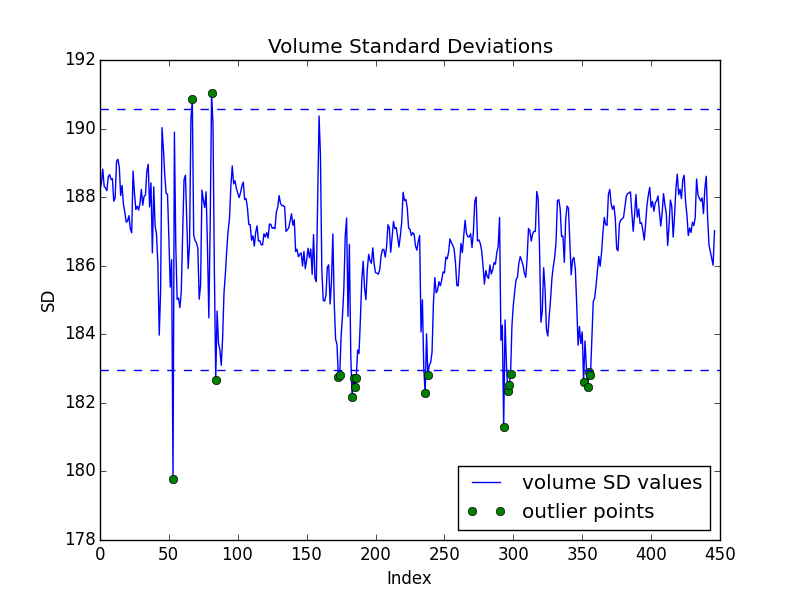
\includegraphics[width=.8\linewidth]{std_plt.png}
  \captionof{figure}{Standard deviation}
  \label{fig:test3}
\end{minipage}%
\begin{minipage}{.5\textwidth}
  \centering
  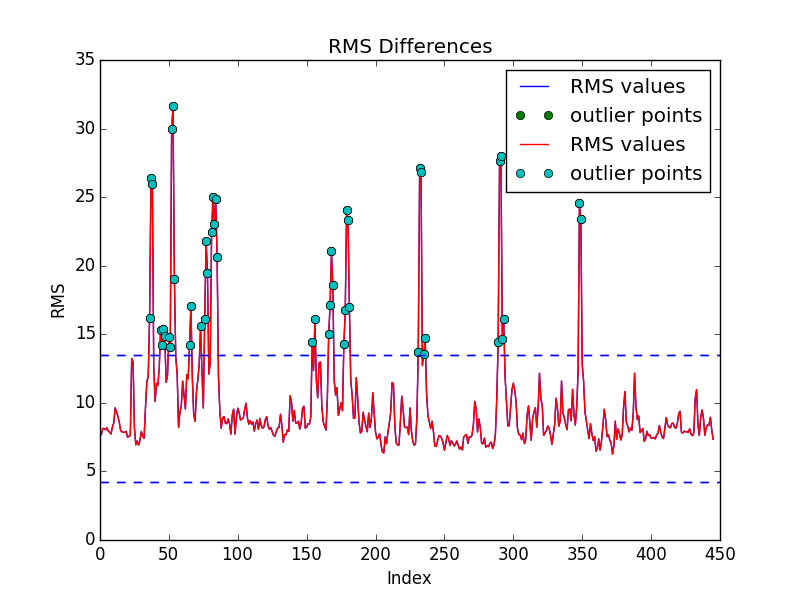
\includegraphics[width=.8\linewidth]{rms_outliers.png}
  \captionof{figure}{RMS(root mean squared differences)}
  \label{fig:test4}
\end{minipage}
\end{figure}


\subsubsection{Spatial Smoothing}
\par Our most preliminary step in preparing the data was to smooth each fMRI image by using a Gaussian Filter function from \texttt{SciPy}  (\texttt{ndimage.filters.gaussian\_filter}) to essentially blur the image slightly. This helps correct for noise which has been shown to be approximately random, voxel-independent, and centered around zero, thus permitting statistical requirements of the Gaussian filter. The Gaussian filter also maintains gradients in detected activity so spatial correlations are preserved, still allowing us to determine regions of brain activation for different concepts and words. This is significant for the purposes of increasing signal-to-noise ratio.
\par Multiple values of the Full Width at Half Maximum (FWHM) filter parameter were tested, with 3mm being selected as the ideal parameter for balance between adequately smoothing regions while maintaining definition of high-activity regions.

\begin{figure}[H]
\centering
\begin{minipage}{.5\textwidth}
  \centering
  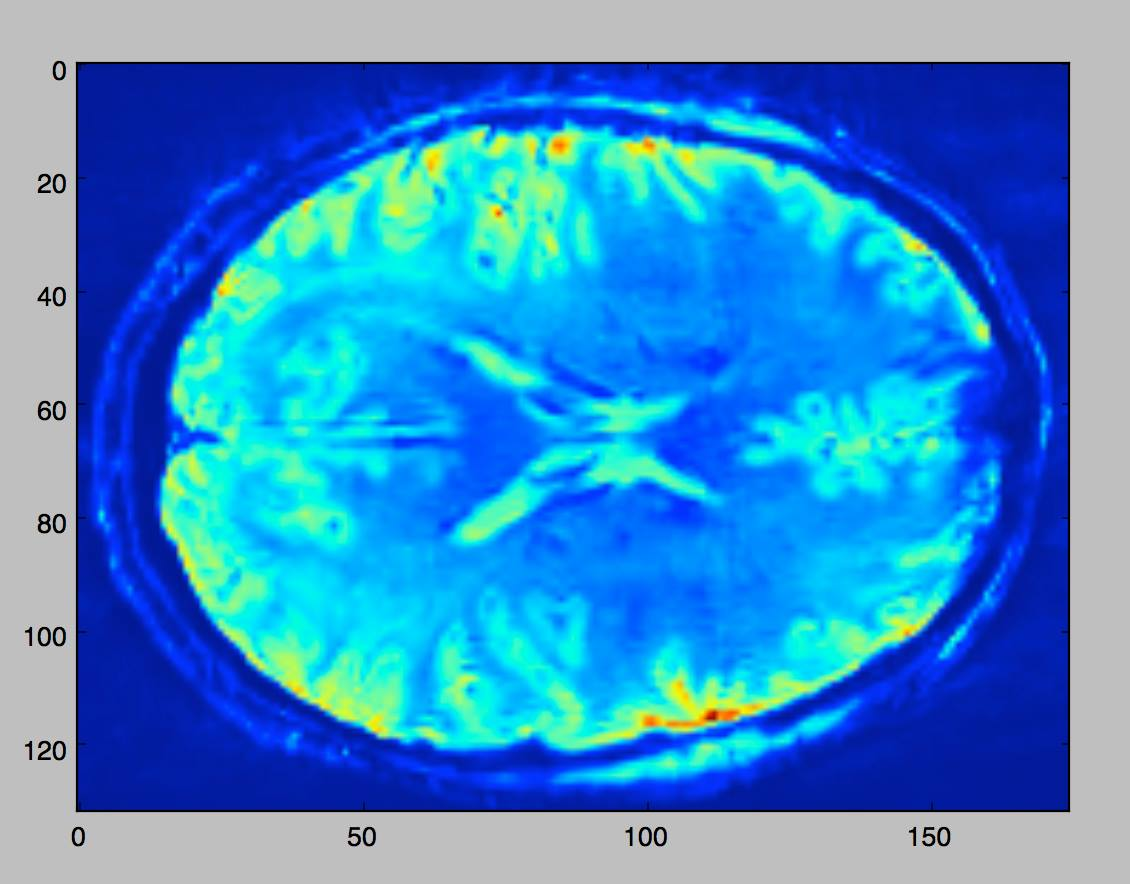
\includegraphics[width=.8\linewidth]{unsmoothed.jpg}
  \captionof{figure}{Raw fMRI image}
  \label{fig:test1}
\end{minipage}%
\begin{minipage}{.5\textwidth}
  \centering
  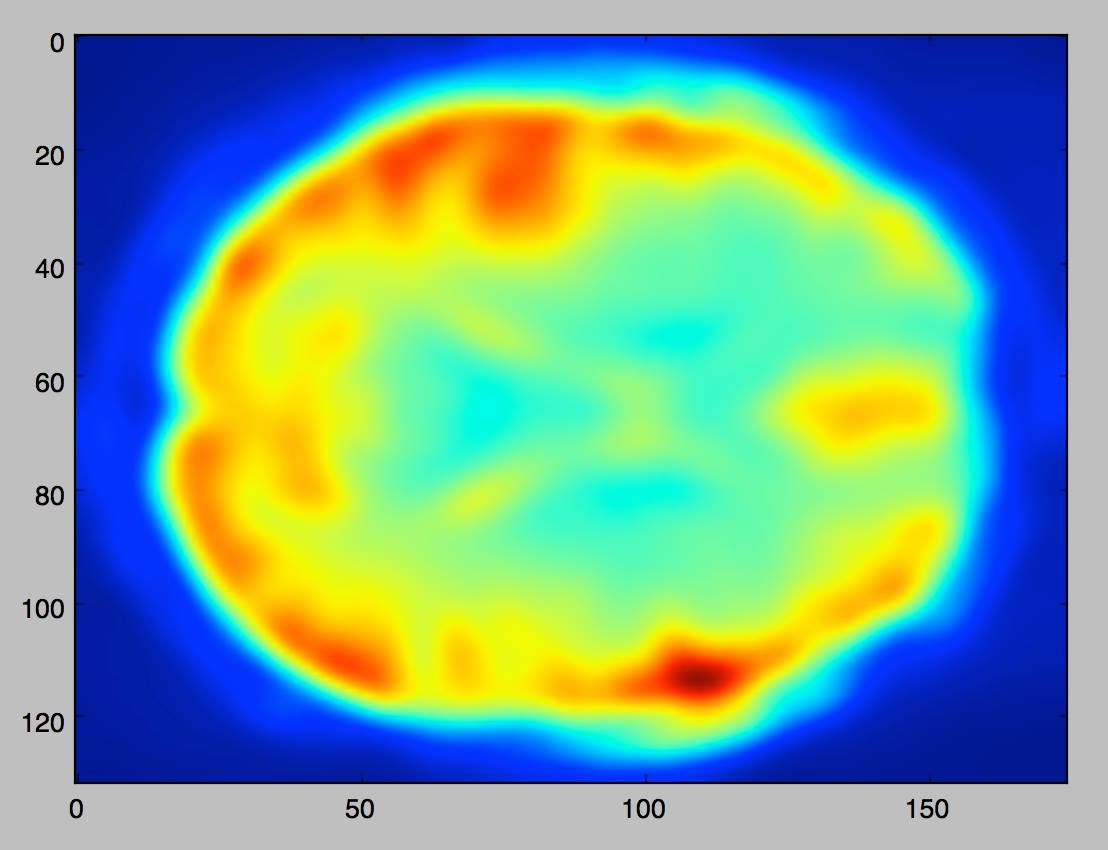
\includegraphics[width=.8\linewidth]{smoothed3mm.jpg}
  \captionof{figure}{Smoothed fMRI image, 3mm}
  \label{fig:test2}
\end{minipage}
\end{figure}

\par Figure 3 and Figure 4 represent a single fMRI image from our data. From a comparison between Figure 3 and Figure 4, notice that many of the sharp edges in the raw fMRI image have been blended with the surrounding areas. The minuscule red regions in the top and bottom areas of Figure 3 have been clearly increased, as well.  

\subsubsection{Temporal Filtering}
\par Given the smoothed images, the signal-to-noise ratio has been improved, equivalent to an amplification of the signal elements. At this point, we thus try to distinguish between the signal and noise and eliminate the noise elements. To this end, signal analyzers utilizing Fast-Fourier Transform (FFT) were used to identify low-frequency noise, and remove it. \texttt{Nitime}'s \texttt{analysis} package existed to help fulfill this task. 
\par The Fast-Fourier Transform	allows you to  
\par Again, as noise is voxel-wise independent, each voxel was analyzed and adjusted individually.

\begin{figure}[H]
\centering
\begin{minipage}{.5\textwidth}
	\centering
	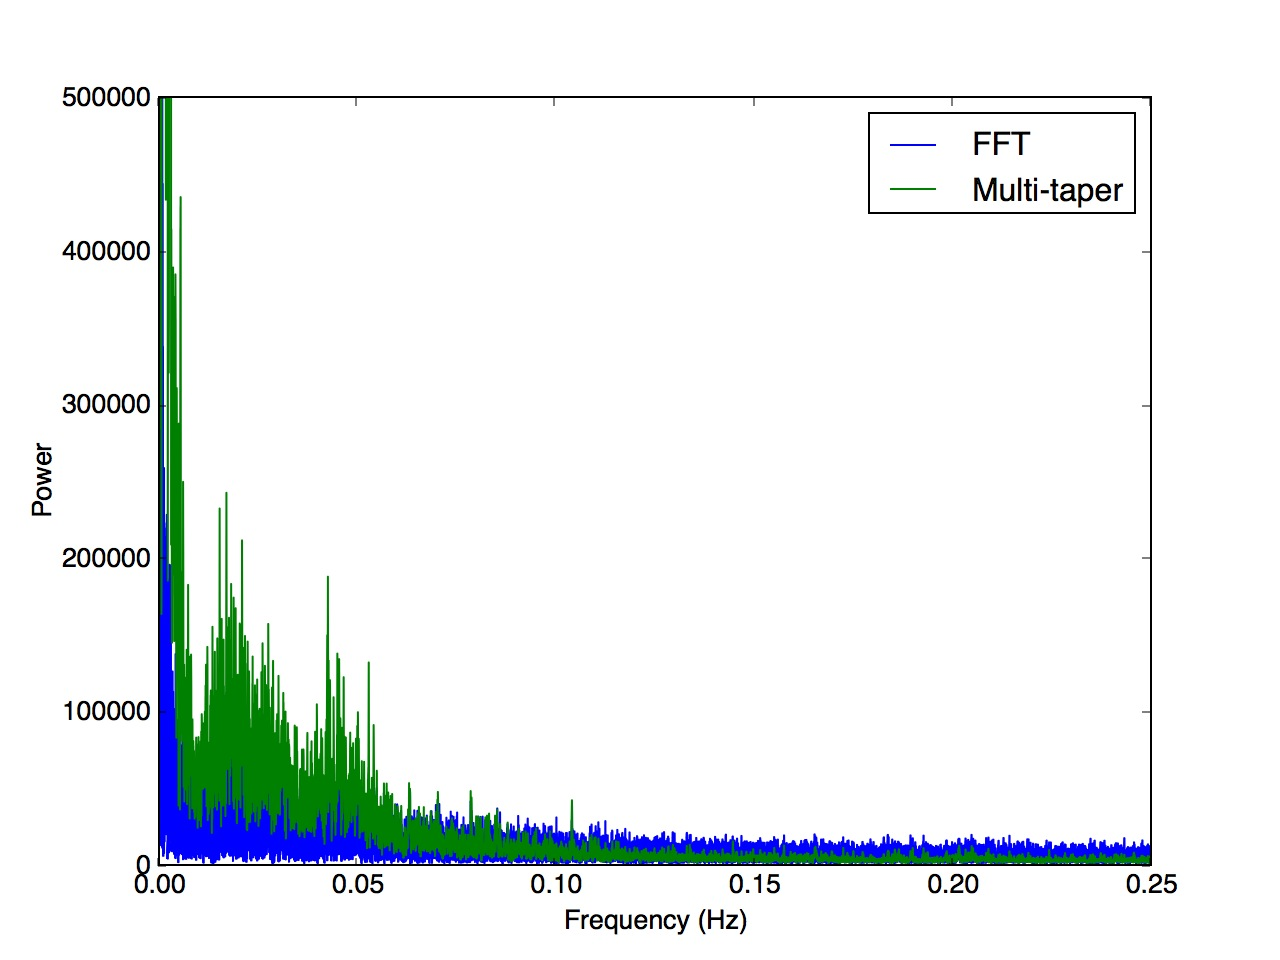
\includegraphics[width=.7\linewidth]{freq_decomp.jpg}
	\captionof{figure}{Voxel Frequency Decomposition}
	\label{fig:test5}
\end{minipage}%
\begin{minipage}{.5\textwidth}
  \centering
  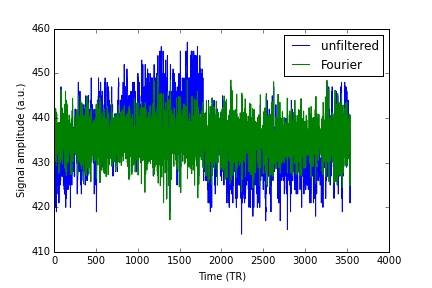
\includegraphics[width=.8\linewidth]{filtered_data.jpg}
  \captionof{figure}{Voxel Filtered Data}
  \label{fig:test1}
\end{minipage}
\end{figure}

\par Figure 7 illustrates the frequency decomposition for a voxel's signal, performed using \texttt{Nitime}'s \texttt{analysis.SpectralAnalyzer} module. There is a huge spike in low-frequency noise, manifesting in the unfiltered signal in Figure 8 as a wave along which the signal drifts. After filtering out this low-frequency noise using \texttt{nitime.analysis.FilterAnalyzer} (post-FFT), there is a noticeable increased in normality of the signal for a single voxel.

\subsubsection{Spatial Filtering}
\par Each of our fMRI scans at each time point occurred in dimensions of 160 x 160 x 30, for a total of 768,000 voxels per time point. With only approximately 3500 time points, our $m\times n$ data matrix becomes a case where $n >> m$ ($n$ voxels as features to describe a time point, $m$ number of timepoints). From a theoretical perspective, this is bad because excessive features promotes overfitting during any sort of analysis by giving repetitive and/or irrelevant features, and exponentially increasing the number of possible solutions (often referred to as \textit{The Curse of Dimensionality}). Practically, it also makes it difficult to perform analyses and machine learning for this volume of data due to hardware limitations. For these reasons, at this stage, we choose to reduce the number of voxels we consider in our analysis.
\par After taking care to amplify signal and remove noise, voxel values at this point reflect true values of BOLD activity. Voxels of interest are those that show significant variance in the subject. Since noisy waves/variation is removed, irrelevant voxels display approximately flat plots. 
\par We determine a boolean mask to apply to our data via taking the top $x$ voxels with highest variance. $x$ values considered were 50,000, 17,000, and 9,000 voxel subsets. These masks were visualized layered on the original image.

\begin{figure}[H]
\centering
\begin{minipage}{.5\textwidth}
  \centering
  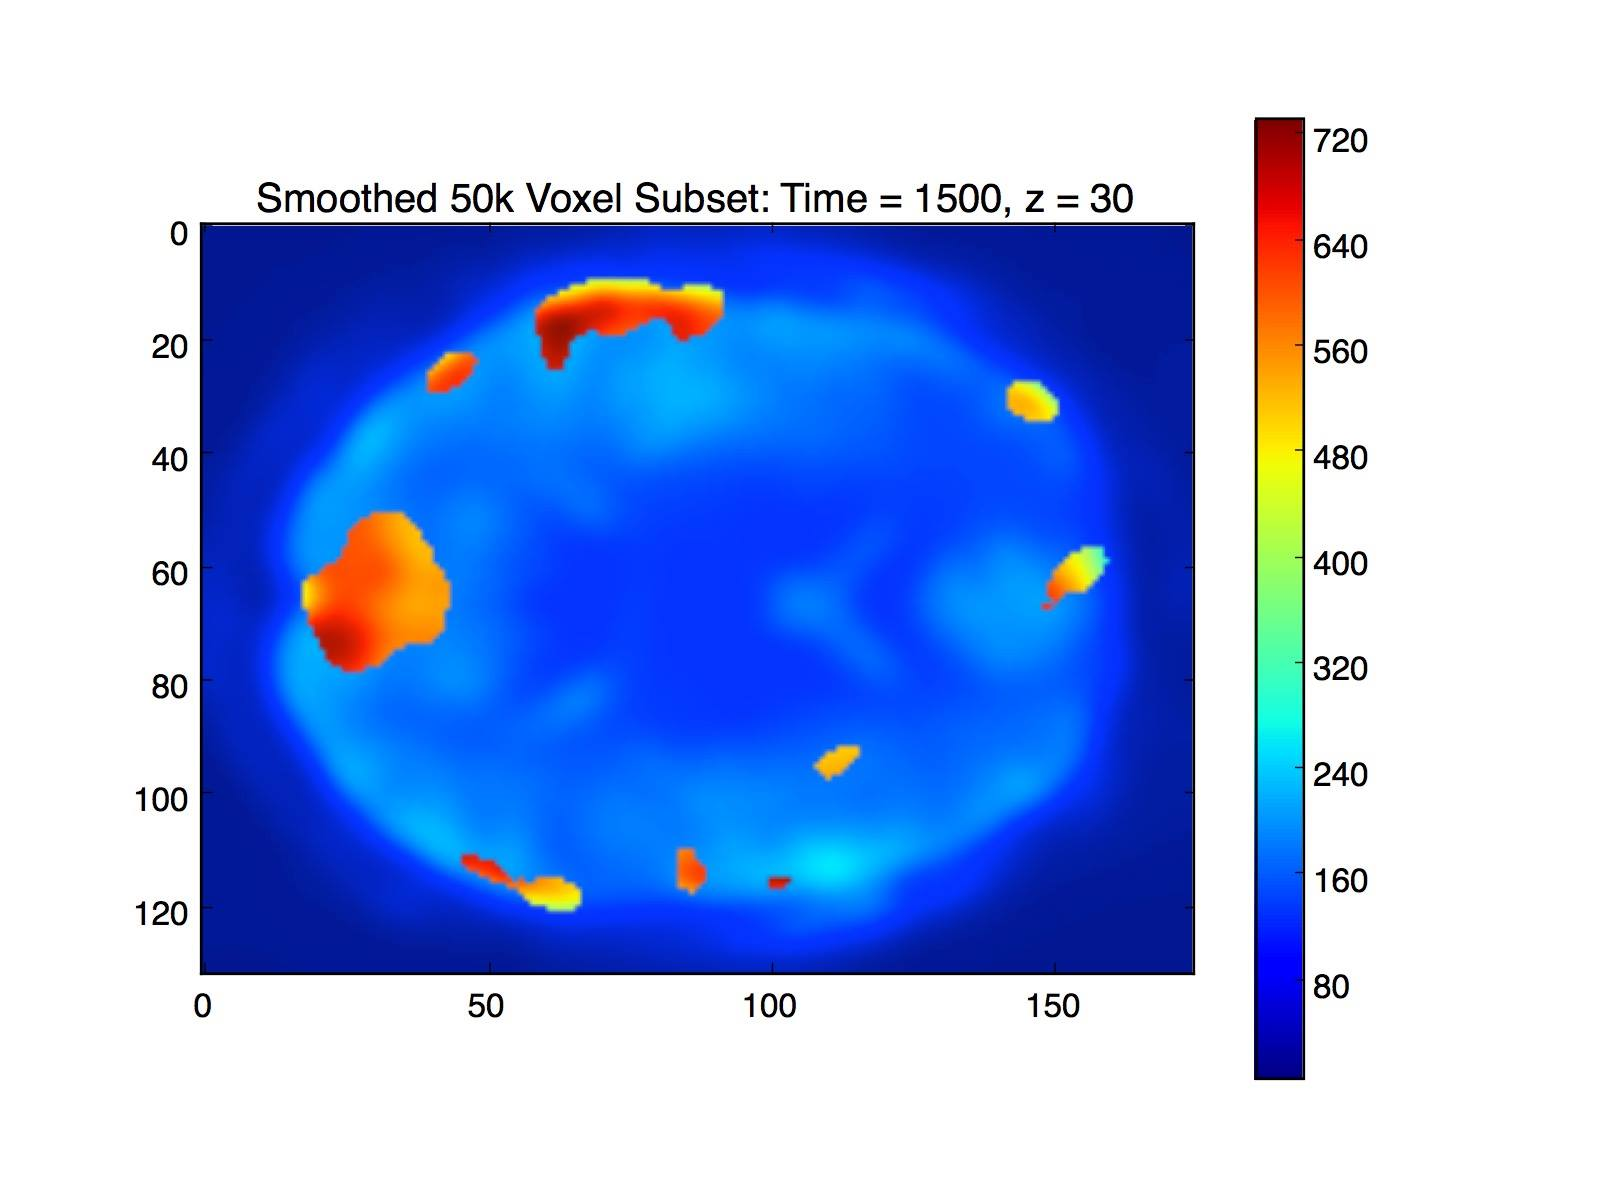
\includegraphics[width=.8\linewidth]{smooth50k.jpg}
  \captionof{figure}{50k mask}
  \label{fig:test1}
\end{minipage}%
\begin{minipage}{.5\textwidth}
  \centering
  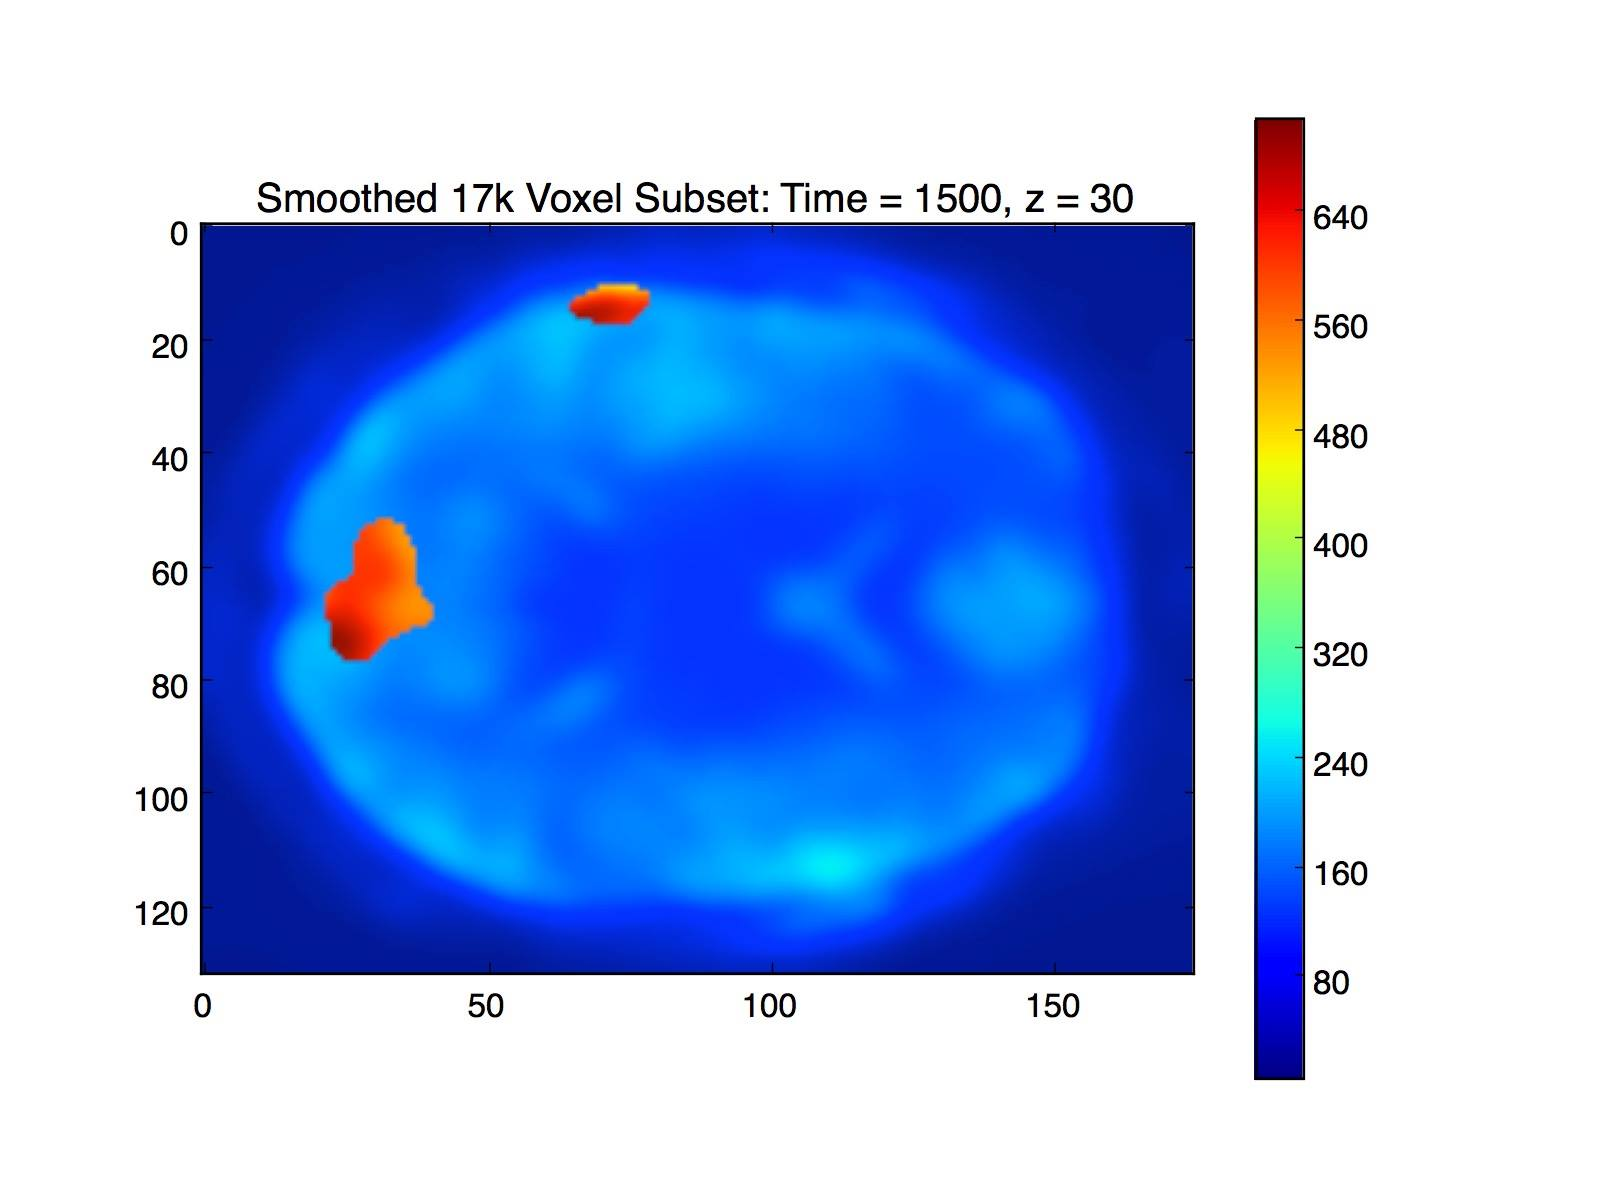
\includegraphics[width=.8\linewidth]{smooth17k.jpg}
  \captionof{figure}{17k mask}
  \label{fig:test2}
\end{minipage}
\begin{minipage}{.5\textwidth}
  \centering
  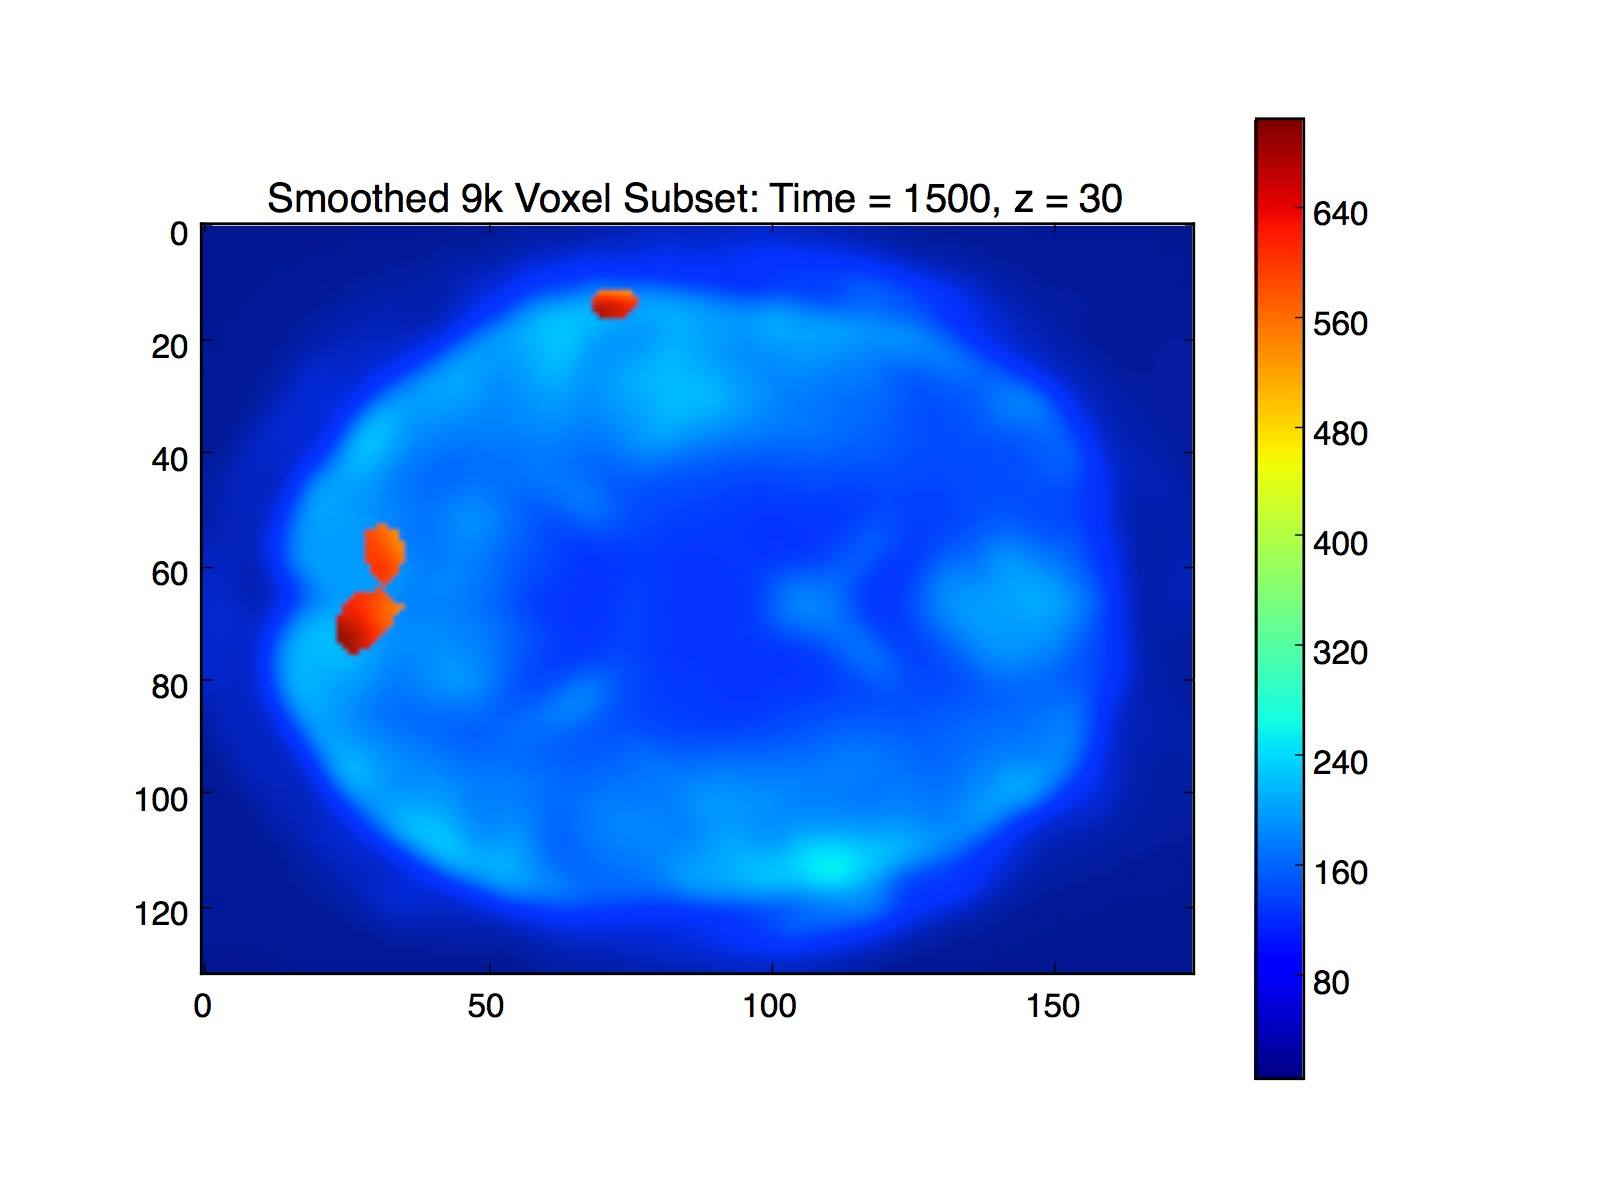
\includegraphics[width=.8\linewidth]{smooth9k.jpg}
  \captionof{figure}{9k mask}
  \label{fig:test2}
\end{minipage}
\end{figure}

\par As the 50k mask retained the most regional variability in brain regions covered, the 50k voxel mask was use in subsequent analyses, applied to the smoothed and filtered data.

\subsubsection{Normalization}
\par To ensure that the data is all scaled equally relative to each other, all of the data was normalized to have 0 mean and a standard deviation of 1, voxel-wise. For each $i$ voxels
$$ Z_i = \frac{X_i - \mu_i}{\sigma_i} $$  
The purpose of this was to ensure that features that span large ranges don't overshadow smaller but more significant features. By putting them on the same scale, this problem is averted.
\begin{figure}
  \centering
  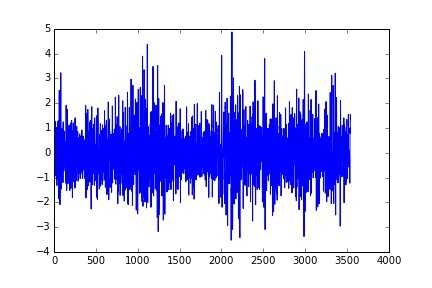
\includegraphics[width=.8\linewidth]{normalized_data.jpg}
  \captionof{figure}{Normalized Voxels}
  \label{fig:test1}
\end{figure}


\subsubsection{Time Lag Correction}
\par For ridge regression, three different time lags(2s,3s,4s) are added to the design matrix to model with the BOLD data.

\break